\documentclass[
	%a4paper, % Use A4 paper size
	letterpaper, % Use US letter paper size
]{jdf}

\addbibresource{references.bib}

\author{Nan Xiao}
\email{nanx@gatech.edu}
\title{CS6750 HCI Summer 2021:\\Project\\Redesign Chatbot Interface of Agoda}

\begin{document}
%\lsstyle

\maketitle

\begin{abstract}
	In this paper, we will redesign the chatbot interface of Agoda. Firstly, we will introduce how to get to the Agoda chatbot interface. Secondly, we will plan and execute the initial needfinding to understand the weakness of the existing interface and what features the interface is expected to have. Thirdly, we will perform a heuristic evaluation on the existing interface to understand the pros and cons and the reasons. Fourthly, we will conduct the redesign of the interface using the wireframe prototype. Fifthly, we will justify the redesign and explain how the redesigned interface addresses the issues raised in initial needfinding. Finally, we will discuss the evaluation plan of the redesigned interface.
\end{abstract}

\section{Introduction}
Customer service is very costly in the travel domain, so most of the OTA (Online Travel Agent) will have a Chatbot interface as a customer service channel to automatically answer some of the customer queries. Since chatbot is generally available on consumer websites, users are not unfamiliar with such interfaces. 

To access Agoda Chatbot, one need to follow the below steps as shown in \textit{\textbf{Figure 1}}:
\begin{enumerate}
	\item Go to Agoda website (https://www.agoda.com) or open the Agoda mobile app.
	\item Login with your Agoda account.
	\item Go to "More" tab. 
	\item Click "Help Center".
	\item Click the "Assist me" button.
	\item You will be in the Agoda Chatbot interface.
\end{enumerate}

Once the users are on the Chatbot interface, the current servicing flows are predefined. There are 8 categories users can select: "Cancellation", "Name Change", "Add guest", "Booking confirmation", "E-receipt", "Date change", "Hotel contact", "Hotel policies". One can play with the existing customer servicing flows in this Chatbot interface to experience. The Chatbot interface currently has limited functionalities.

\begin{figure}[hbt!]
	\centering
	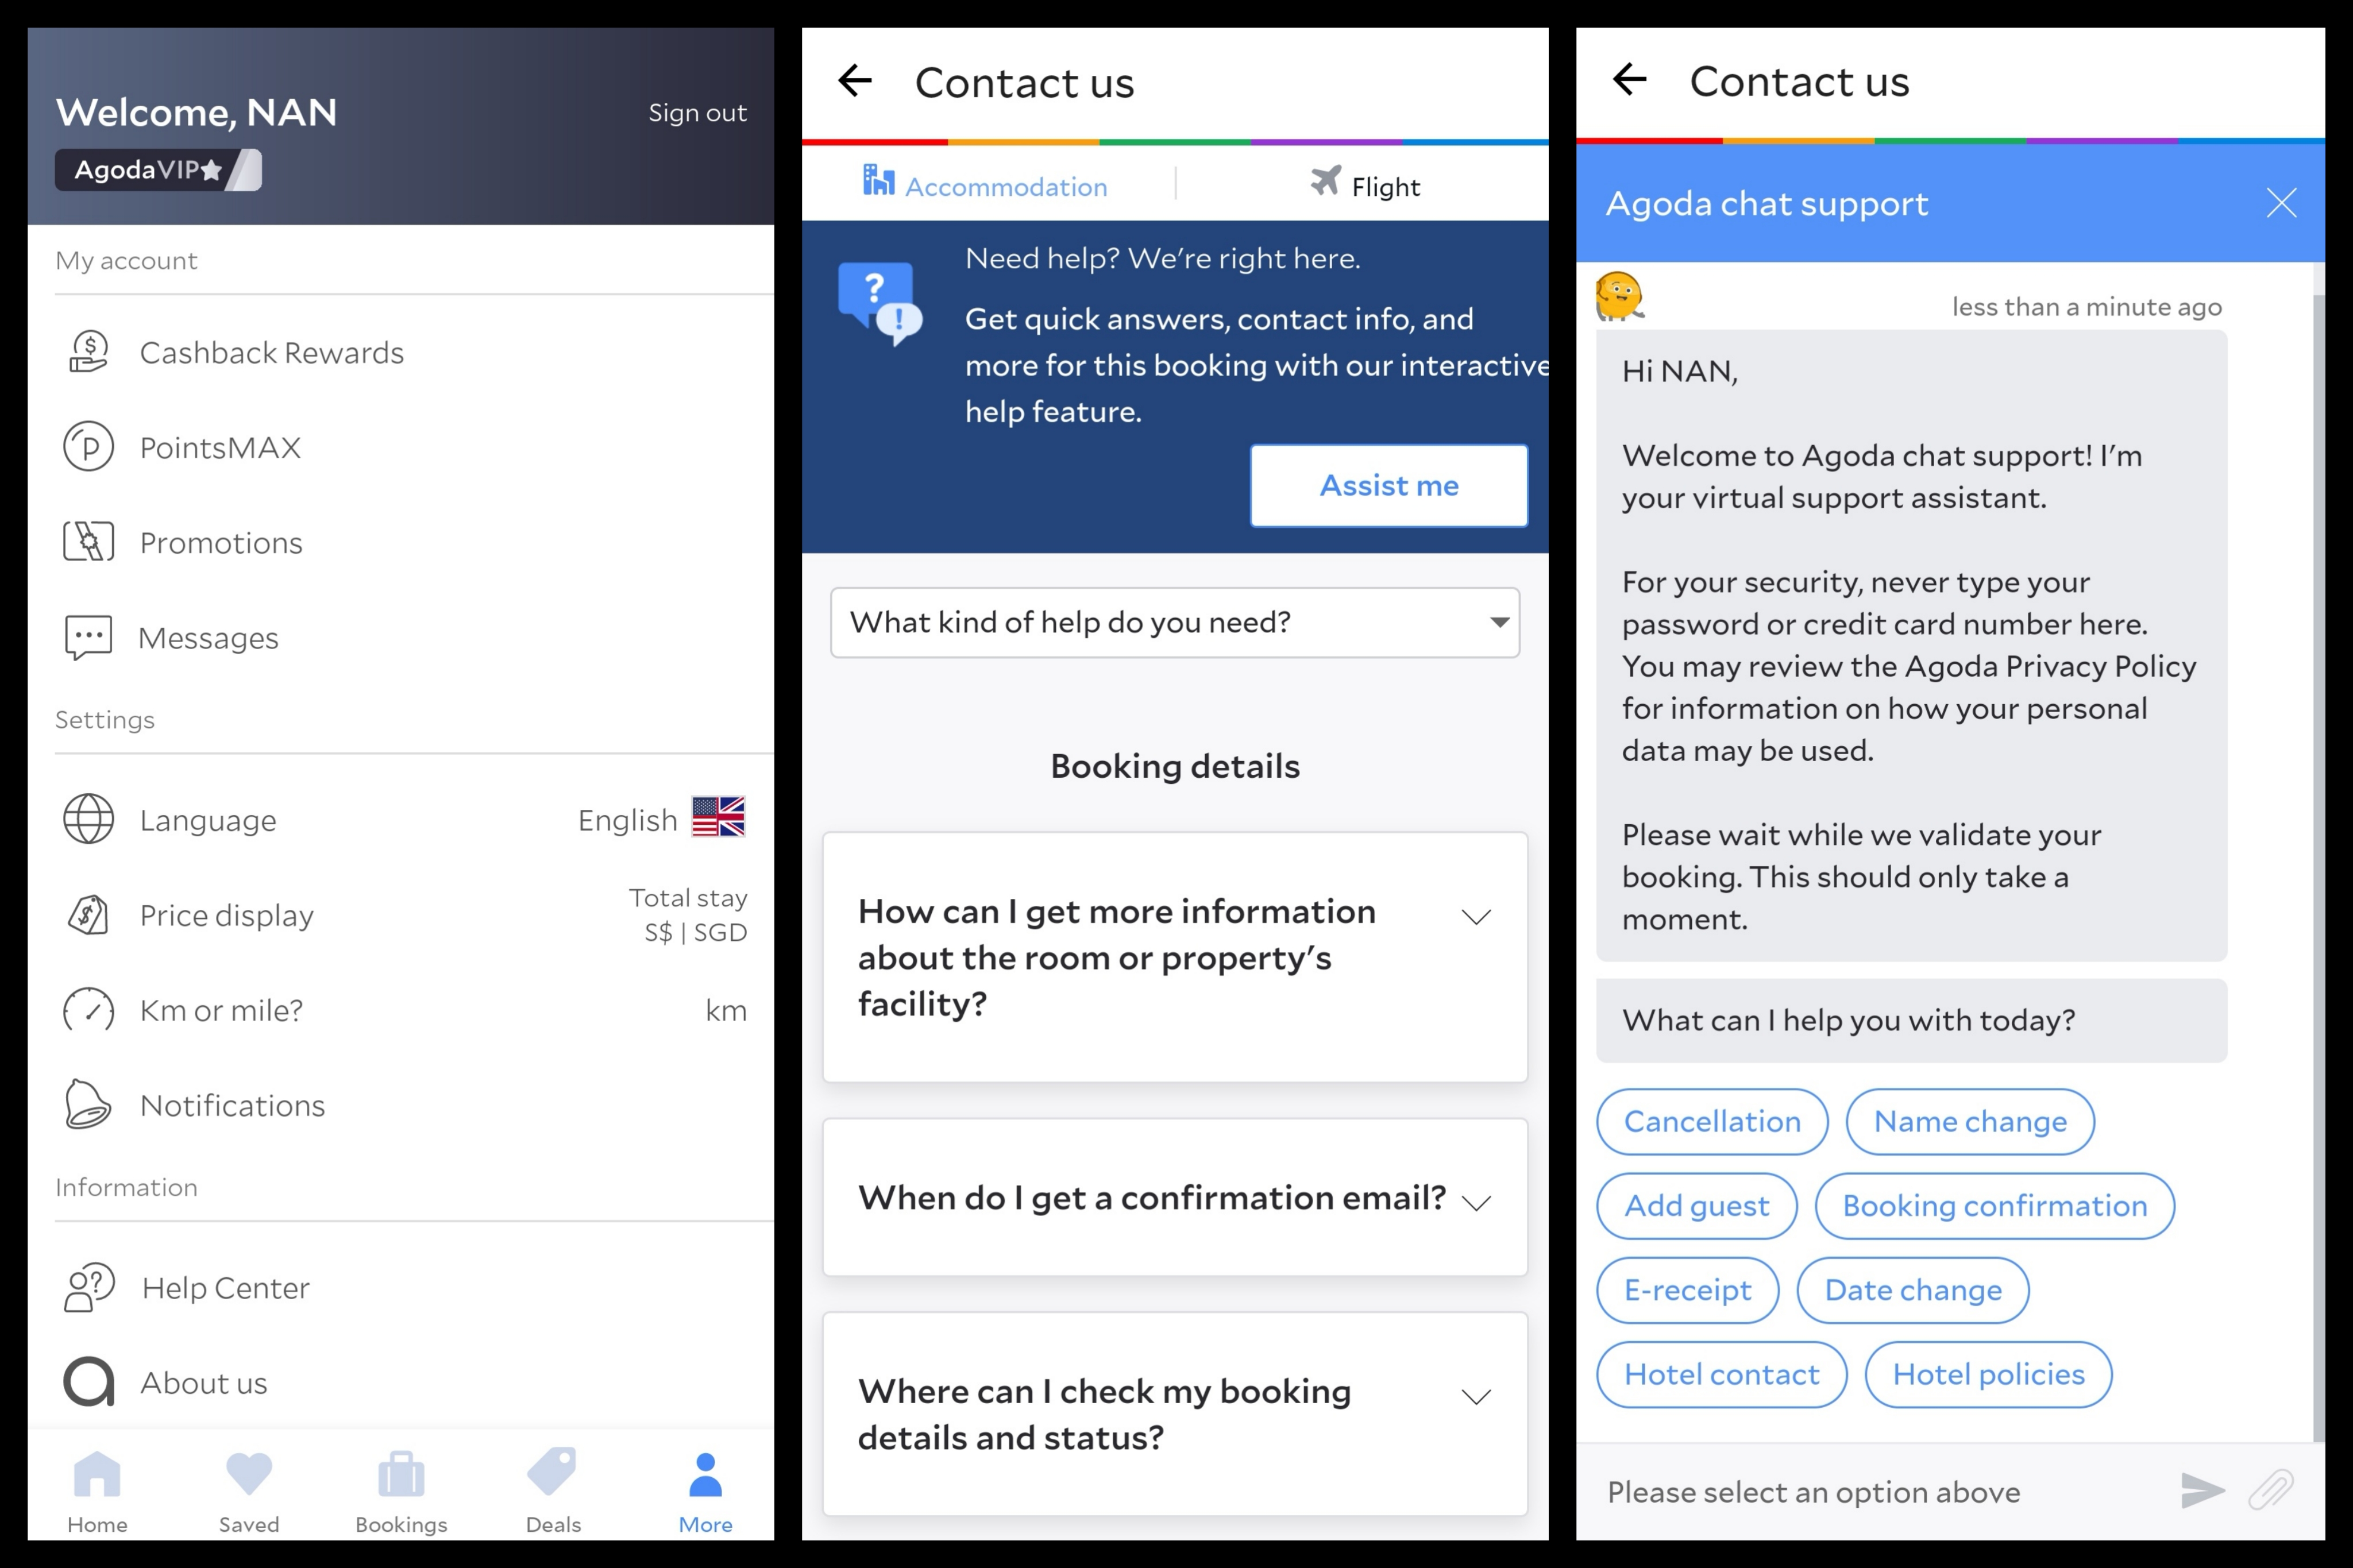
\includegraphics[height=10cm]{jdf-latex/Figures/agoda_existing.jpeg}
	\caption{Existing Chatbot Interface of Agoda}
	\label{fig:wizard}
\end{figure}

\section{Initial Needfinding}
\subsection{Needfinding Approaches and Plans}

To understand the current weakness of the Agoda chatbot interface, \textbf{Interview} and \textbf{Product Review} are chosen to be methods for needfinding. The reason to use Interviews together with Product Reviews is to reduce the bias. \textit{\textbf{Table 1}} summarizes the potential biases and solutions from both methods.

\begin{table}[hbt!]
	\caption{Needfinding Methods Biases and Solutions}
	\small % Reduce font size
	\centering % Centre the table
	\begin{tabular}{L{0.1\linewidth} L{0.2\linewidth} L{0.3\linewidth} L{0.3\linewidth}}
		\textbf{Method} & \textbf{Bias} & \textbf{Reason} & \textbf{Solution} \\
		\toprule[0.5pt]
		Interview & Social Desirability Bias & People tend to agree with interviewer if the questions have certain tendency & Phrase the question neutrally \\
		\midrule
		Product Review & Voluntary Response Bias & People writing product review usually have strong opinions & We need to use Product Review together with Interview \\
	\end{tabular}
\end{table}

Also, through product reviews, we can gather the general issues of the Agoda app, but might not be directly related to the Chatbot interface. We can get more targeted feedback on the Chatbot interface from Interviews.

\subsubsection{Interview plan}
To make surveys more effective, we need to make sure below 5 points (\cite{joyner2016c}):
\begin{enumerate}
	\item Less is more. Ask minimum questions necessary.
	\item Be aware of bias, phase questions in a neutral way.
	\item Tie them to the inventory.
	\item Test it out. Have co-workers test survey questions before sending them out.
	\item Iterate and revise surveys according to the tests.
\end{enumerate}
Below interview questions will be asked for 10 people to gather feedback on the Chatbot interface of the Agoda app. 
\begin{enumerate}
	\item Which app do you use to book hotels when you are travelling?
	\item What do you like about Agoda?
	\item What do you dislike about Agoda?
	\item (After trying the Chatbot interface) What do you like about the interface?
	\item (After trying the Chatbot interface) What do you dislike about the interface?
\end{enumerate}

\subsubsection{Product Review plan}
We will collect and review the top 50 reviews from both Google Play Store and Apple App Store. Because these two stores are the most popular sources for the users to access the Agoda app. There are 480K downloads from Play Store and 34.1K ratings from the App store. These are great places to find out what people dislike about the app, especially in the customer service sector. We will use the redesigned Chatbot interface to address those issues.

\subsection{Needfinding Conclusion - Results and Summary}
\subsubsection{Summary and Analysis - Interviews \& Product Reviews}
For the interview result, all people know the Agoda app, since it is one of the most popular travel apps in the region. The major benefit of using the Agoda app is that people can easily book a hotel through the platform. And the major concern of the app is that the app may not offer the best hotel price. In terms of the Chatbot interface, interviewees generally like the feature that it shows the capabilities upfront. People thus understand what can be done through Chatbot. The major concern of the Chatbot interface is that most of the scenarios that users need help with are not addressed by the existing Chatbot interface. For example, if they want to know if the hotel has a 24hrs reception, or whether it supports quarantine, the current Chatbot interface cannot answer those questions.

For the product reviews, the common things people like are "Website is very easy to use", "User friendly", and "Great value for money". People like the ease of use of the existing interface. But seldom do people mention the chatbot interface. It may indicate that the entry of chatbot is hard to find. When we look at the common thing people dislike about Agoda, they are "Poor customer service and site issues", "There is no way to get help from Agoda", or "Tried to contact Agoda for help but the BOT directing us was useless". People use app reviews as a channel for complaints. The major reason for the complaints is due to poor customer service. And people do feel the Chatbot is useless if it cannot address the users' issues and is not able to connect the users to real agents in the interface.

\subsubsection{Data Inventory - Interviews \& Product Reviews}
These are the questions we want to answer through our needfinding exercises: (\cite{joyner2016d})
\begin{itemize}
    \item Who are the users?
    \item Where are the users?
    \item What is the context of the task?
    \item What are their goals?
    \item What do they need?
    \item What are their tasks?
    \item What are their subtasks?
\end{itemize}

\textit{\textbf{Table 2}} summarizes data inventories in the Interviews \& Product Reviews method.

\begin{table}[hbt!]
	\caption{Data Inventory - Interviews \& Product Reviews}
	\small % Reduce font size
	\centering % Centre the table
	\begin{tabular}{L{0.1\linewidth} L{0.1\linewidth} L{0.1\linewidth} L{0.15\linewidth} L{0.15\linewidth} L{0.2\linewidth}}
		\textbf{Who} & \textbf{Where} & \textbf{Context} & \textbf{Goal} & \textbf{Need} & \textbf{Tasks}\\
		\toprule[0.5pt]
		Users pre-booking & Home & Plan and book hotels & Successfully book hotels on Agoda app & Easily find relevant hotel information through Chatbot interface & Find Chatbot interface, ask questions, follow suggested flow, get answers \\
		\midrule
		Users post-booking & Destination & Need to check-in hotels & Get a receipt for hotel booking & Chatbot to provide steps to get e-receipt & Find Chatbot interface, ask questions, follow suggested flow, get e-receipt \\
		\midrule
		Users post-booking & Destination & Hotel has no room to offer & Cancel booking and find a nearest hotel & Cancel existing booking and make a new booking & Find Chatbot interface, ask questions, follow suggested flow, get real agent chat \\
	\end{tabular}
\end{table}
\clearpage

\section{Heuristic Evaluation}
In this section, we will perform the heuristic evaluation to evaluate the existing chatbot interface. We have 15 design principles to evaluate as summarized in \textit{\textbf{Figure 2}}.(\cite{joyner2016e}) We will discuss areas the current interface meet the design principles and areas it does not.
\begin{figure}[hbt!]
	\centering
	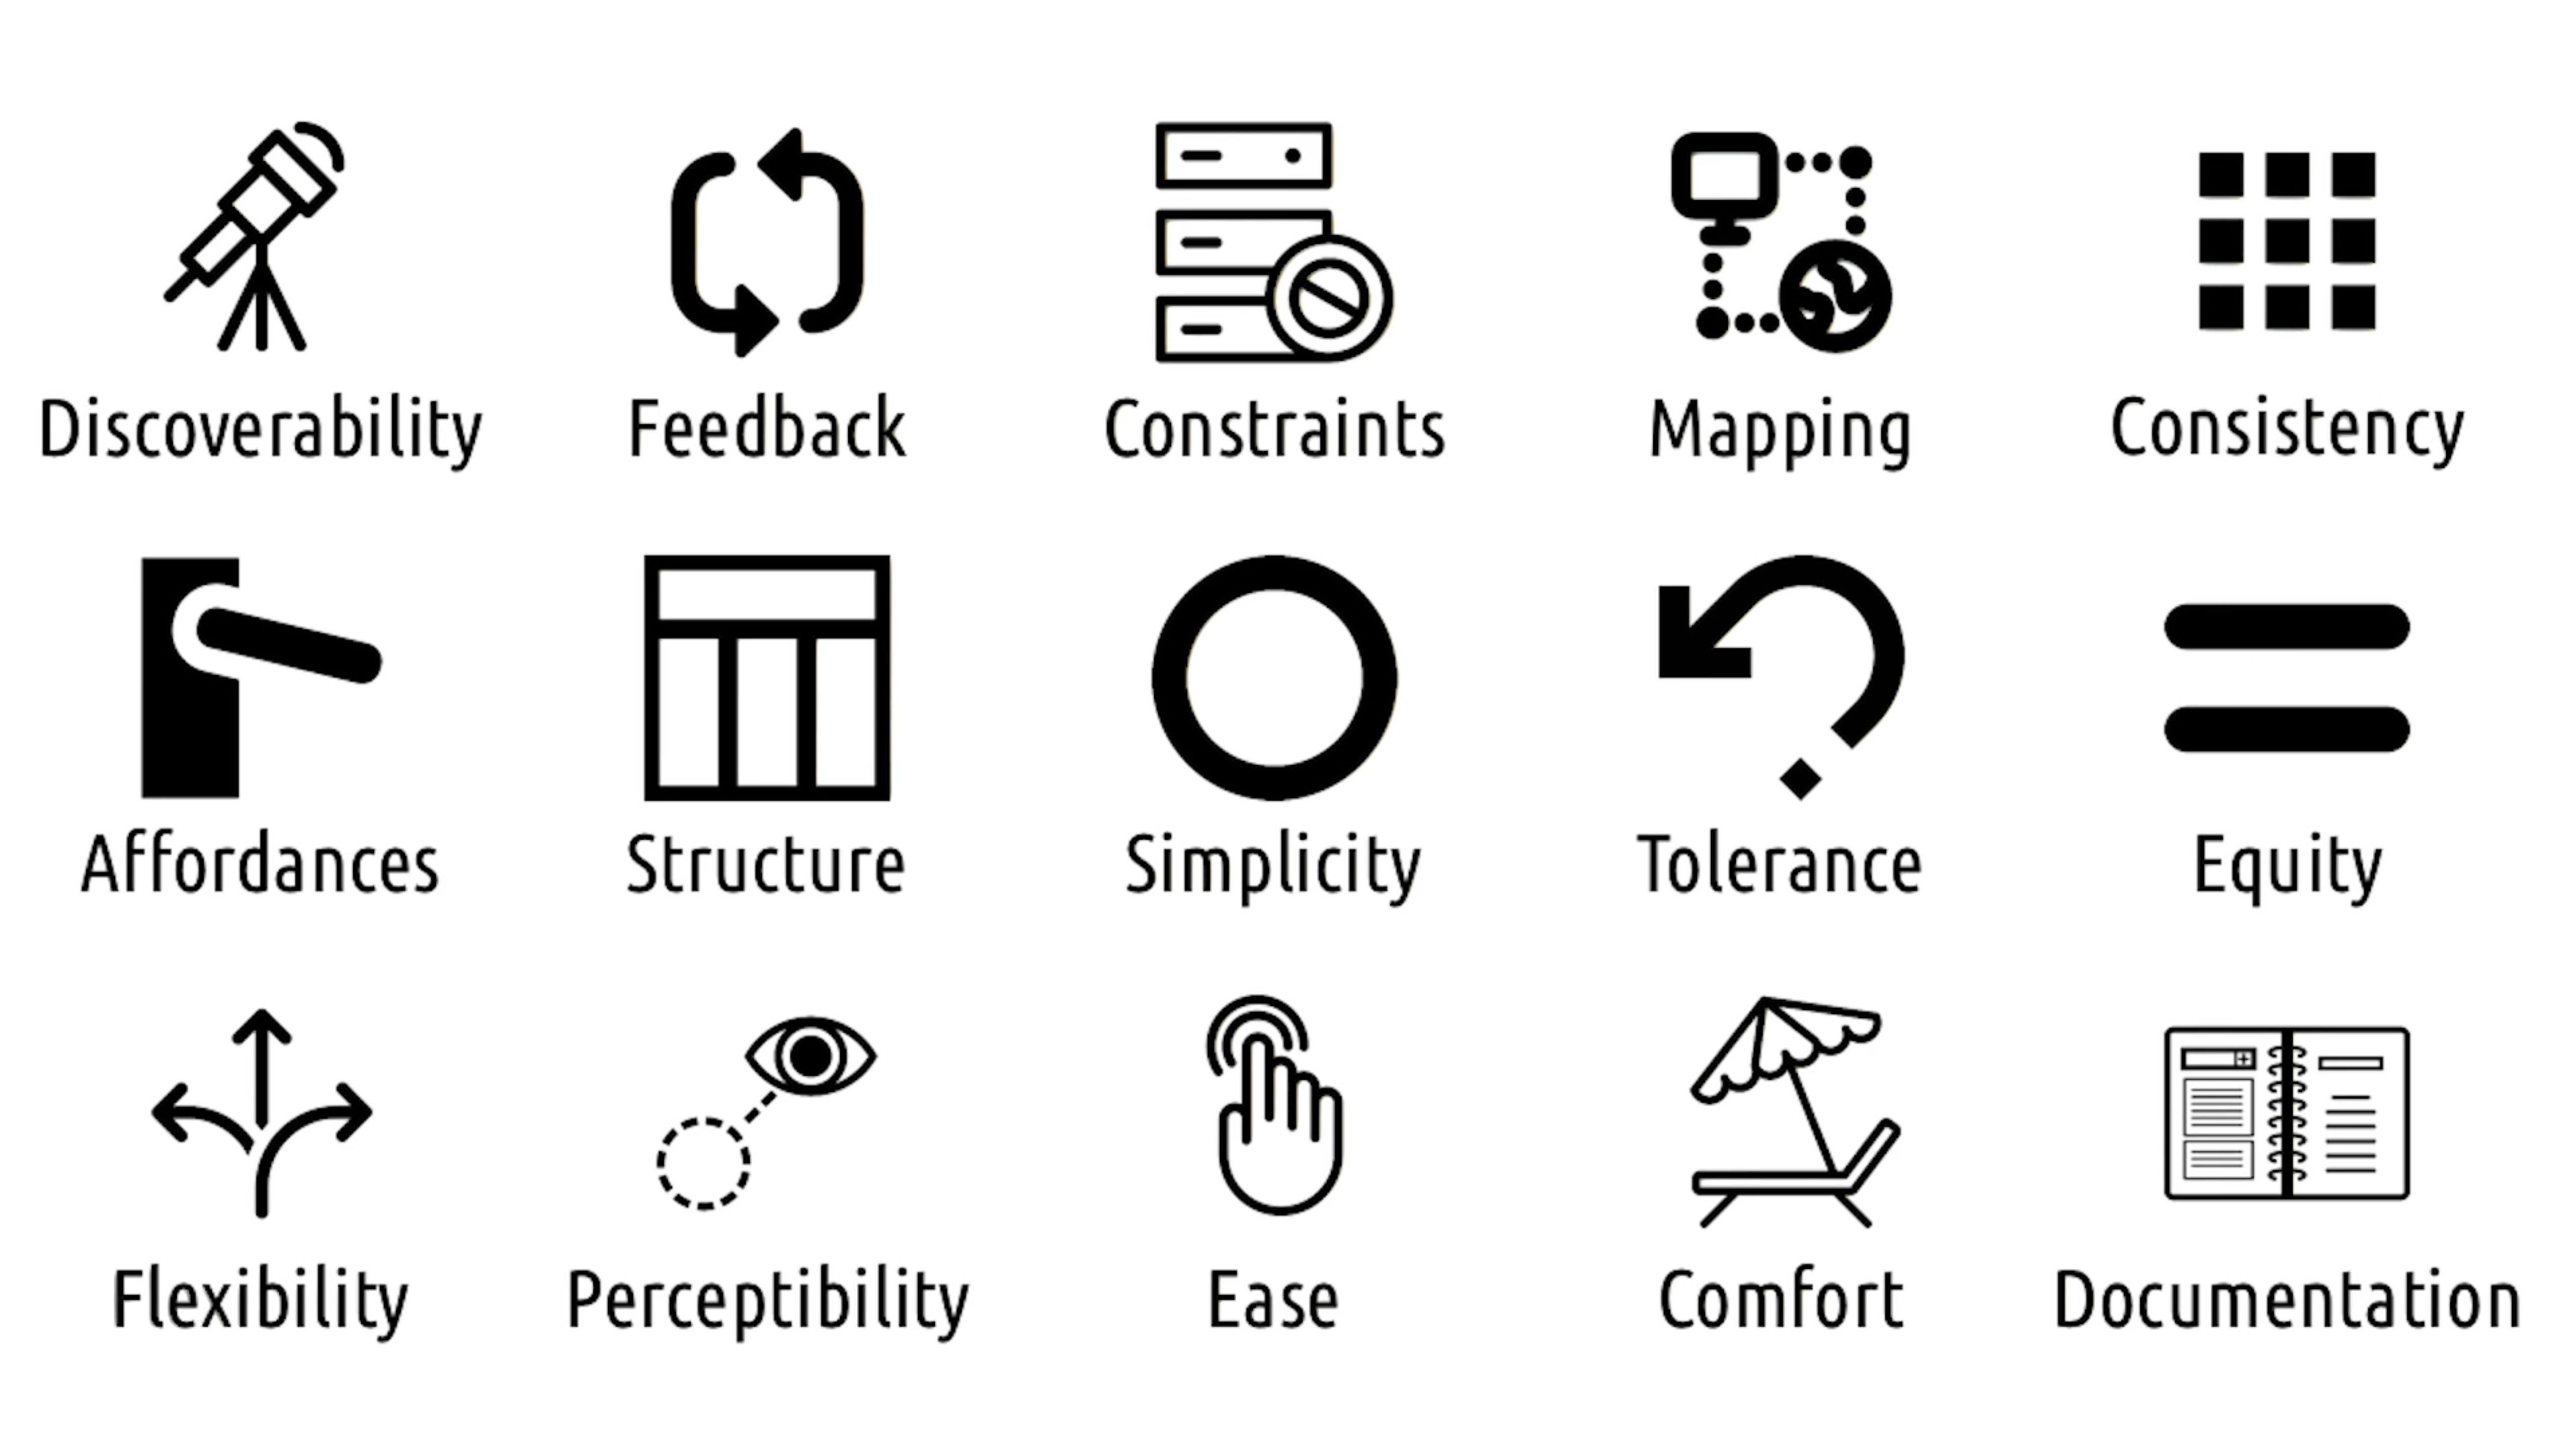
\includegraphics[height=6cm]{jdf-latex/Figures/Heuristic Evaluation.png}
	\caption{15 Design principles for Heuristic Evaluation}
	\label{fig:wizard}
\end{figure}

\subsection{What works well and What makes it work well}
We will summarize what works well and why in the \textit{\textbf{Table 3}}
\begin{table}[hbt!] % [h] forces the table to be output where it is defined in the code (it suppresses floating)
	\caption{What works well and why for existing chatbot interface}
	\small % Reduce font size
	\centering % Centre the table
	\begin{tabular}{L{0.35\linewidth} L{0.15\linewidth} L{0.4\linewidth}}
		\textbf{What works well} & \textbf{Design Principle} & \textbf{What makes it work well} \\
		\toprule[0.5pt]
		Users are well informed about what's going on & Perceptibility & The conversation flow keeps user understand the context, and the user gets fast response \\
		\midrule
		Users will not able to generate wrong input & Constraints & Users can only press predefined intentions buttons \\
		\midrule
		The interface is simple and easy for the user to understand & Simplicity & Interface is clean and with only necessary information \\
		\midrule
		The interface is simple and easy for the user to understand & Ease & Users can click buttons provided and get into the serving flow \\
		\midrule
		Users can use the chatbot interface on mobile or desktop & Comfort & The chatbot interface uses different designs to fit for both mobile and desktop screens \\
		\midrule
		Users speaking different language can all use the chatbot interface & Equity & The chatbot interface support multiple languages \\
	\end{tabular}
\end{table}
\subsection{What does not work well and Why does not it work well}
We will summarize what does not work well and why in the \textit{\textbf{Table 4}}

\begin{table}[hbt!] % [h] forces the table to be output where it is defined in the code (it suppresses floating)
	\caption{What does not work well and why for existing chatbot interface}
	\small % Reduce font size
	\centering % Centre the table
	\begin{tabular}{L{0.35\linewidth} L{0.15\linewidth} L{0.4\linewidth}}
		\textbf{What does not works well} & \textbf{Design Principle} & \textbf{Why does not it work well} \\
		\toprule[0.5pt]
		Users are hard to find chatbot interface & Discoverability & To access chatbot interface, one needs to go through multiple pages \\
		\midrule
		The normal user input is greyed out and users will be confused by the interface & Affordance & The interface looks like the normal chatting interface, but users are not allowed to key in free text\\
		\midrule
		Users are not able to make mistakes or ask wrong questions & Tolerance & The interface fixes the possible buttons and leave no room for users to make free questions \\
		\midrule
		Users are not able to ask the real issues they are facing other than the predefined 8 intentions & Flexibility & Free text input is disabled by the interface, there is no place to key in\\
		\midrule
		Users will be confusing about what the chatbot interface can do & Consistency & Many other major industry leaders allow the user to key in free text and transfer to real agents \\
		\midrule
		The interface looks like a chat interface but it only allows follow the pre-defined flow & Mapping & Users would expect to chat in a chatbot interface, but the interface does not provide that functionality \\
		\midrule
		Users have no instruction or documentation to follow if the chatbot fails & Documentation & There is no clear instruction to guide users to real agents if the chatbot fails to serve the users \\
		\midrule
		The feedback is not helpful if the chatbot does not understand the input query & Feedback & For the scenarios like chatbot cannot understand users queries many times, it should transfer to real agent \\
		\midrule
		No structure is used in the current design & Structure & There is no structure information to display in the frontend\\
		\midrule
		Novice users may not need to access chatbot to solve their issues & Expert Blindspot  & There should be instructions to guide novice users to read FAQ first before trying the chatbot interface \\
		\midrule
		Users can be frustrated if they are trying to get in touch with a real agent & Learned Helplessness & The users will not reach the real agent no matter what they try, the interface does not provide an "exit" option for the user using chatbot \\
	\end{tabular}
\end{table}
\clearpage

\section{Interface Redesign}
In this section, we will redesign the chatbot interface using \textbf{high-fidelity wireframe prototype}. The interface will be designed to address the data inventories in section 2. Comparing to the existing interface, the redesign will allow users to key in free text to get the answers. Also, the new interface will auto-complete the user inputs, like when you are typing questions in Google. If the Chatbot knows the user intents, it will guide the user to get the answers. If not, the Chatbot will be transferred to a real agent after failing to serve the customer 3 times. The overall user journey in the redesigned chatbot interface is shown in the \textit{\textbf{Figure 3}}

\begin{figure}[hbt!]
	\centering
	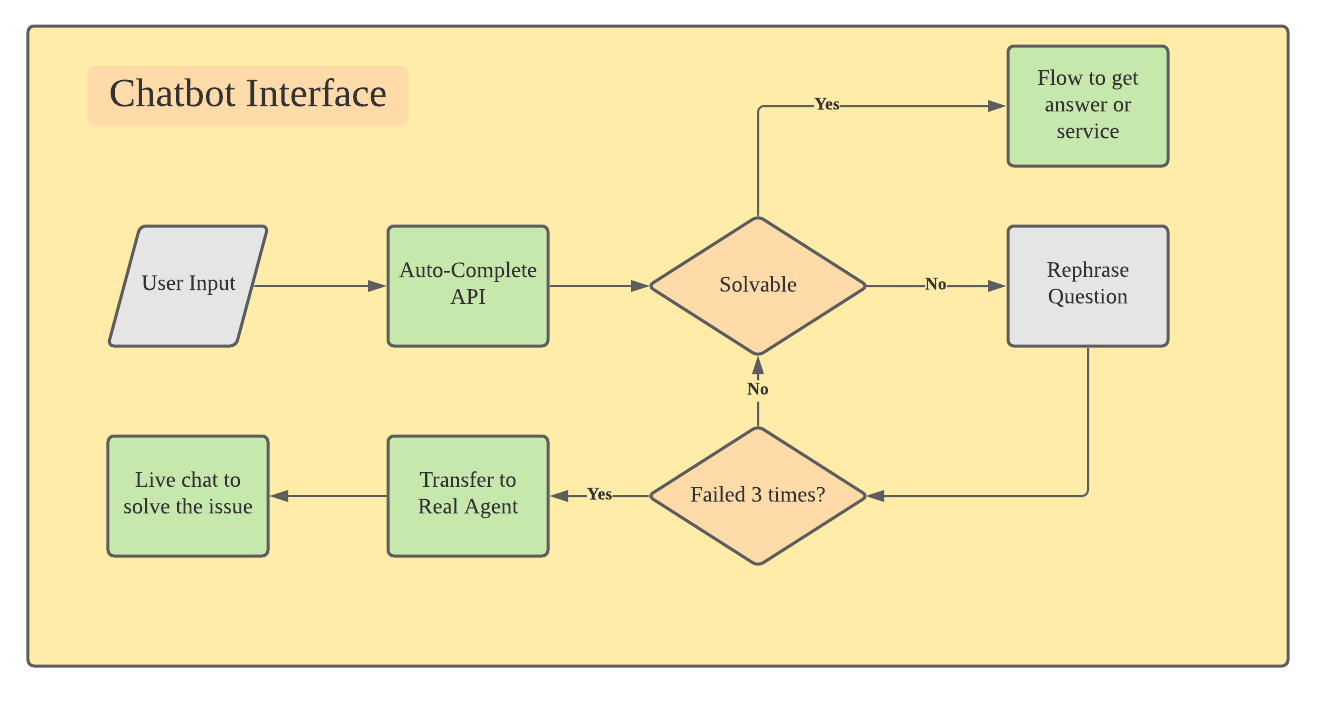
\includegraphics[height=7cm]{jdf-latex/Figures/Chatbot Sandbox.png}
	\caption{Overall Flowchart of the redesigned chatbot interface}
	\label{fig:wizard}
\end{figure}

\subsection{User Journey of Solvable Issue on Chatbot Interface}
As shown in \textit{\textbf{Figure 3}}, users would be able to get the desired answers through the redesigned chatbot interface. The interface will have an auto-complete function like Google to help the user finish the question. Then the interface will suggest users follow steps to have the information they need.

\begin{figure}[hbt!]
	\centering
	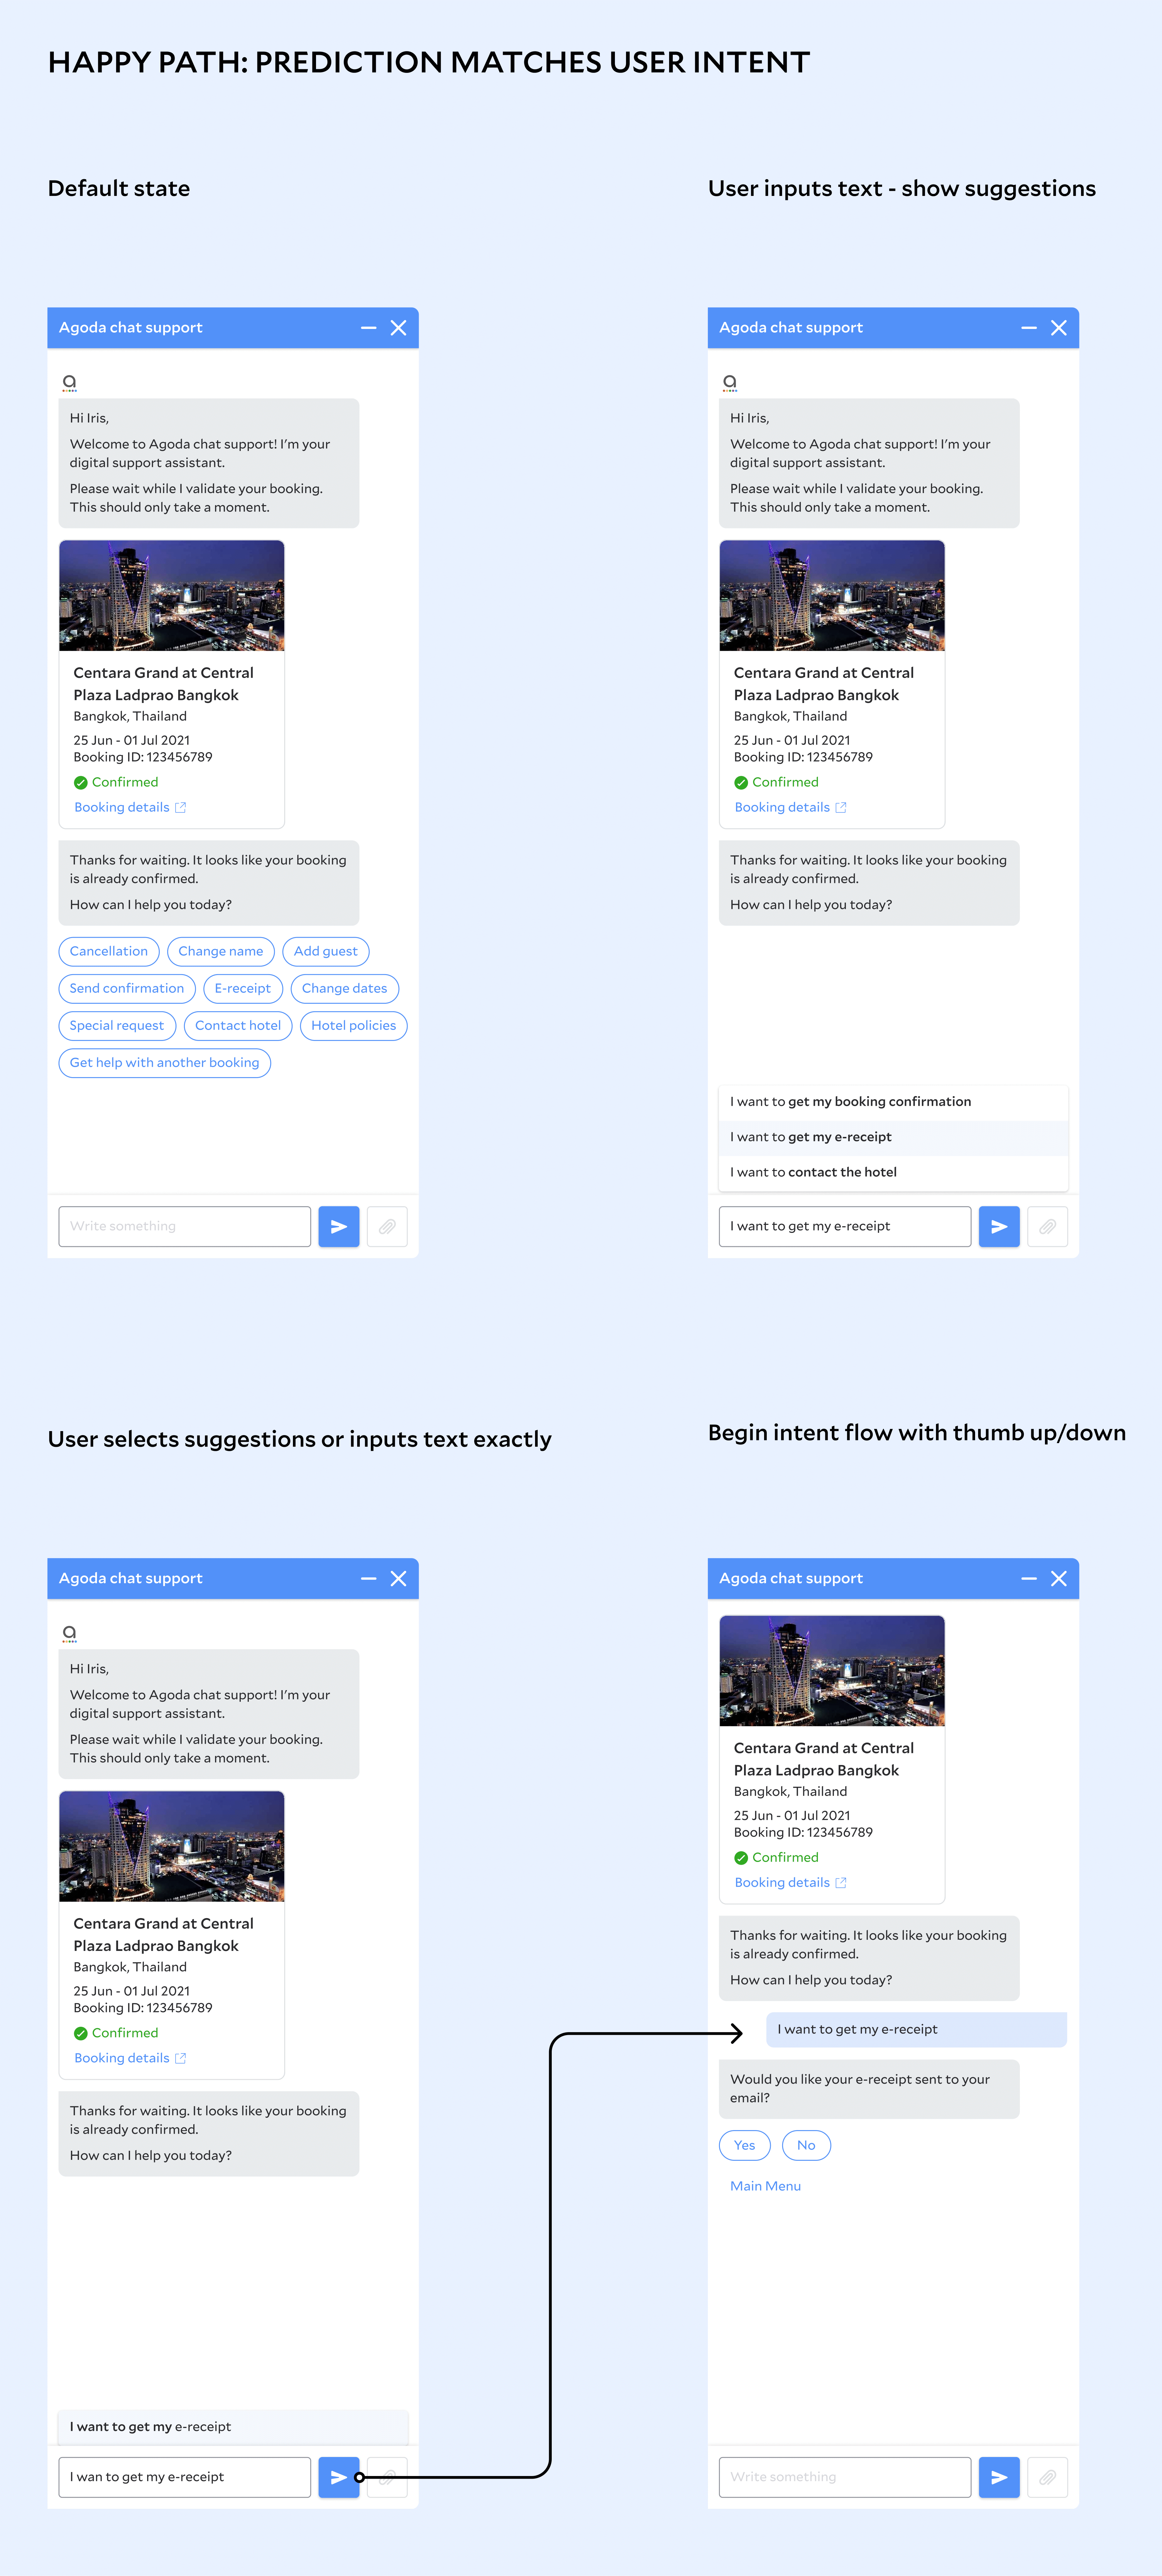
\includegraphics[height=21cm]{jdf-latex/Figures/prototype1.png}
	\caption{User journey to get e-receipt for hotel booking}
	\label{fig:wizard}
\end{figure}

\subsection{User Journey of Unsolvable Issue on Chatbot Interface}
As shown in \textit{\textbf{Figure 4}}, users will be asked to rephrase the question if the Chatbot cannot understand the intent. After 3 times failures, the Chatbot may not have the capability to understand the complex user query, then the user would be able to connect to the real agent to solve the issue.

\begin{figure}[hbt!]
	\centering
	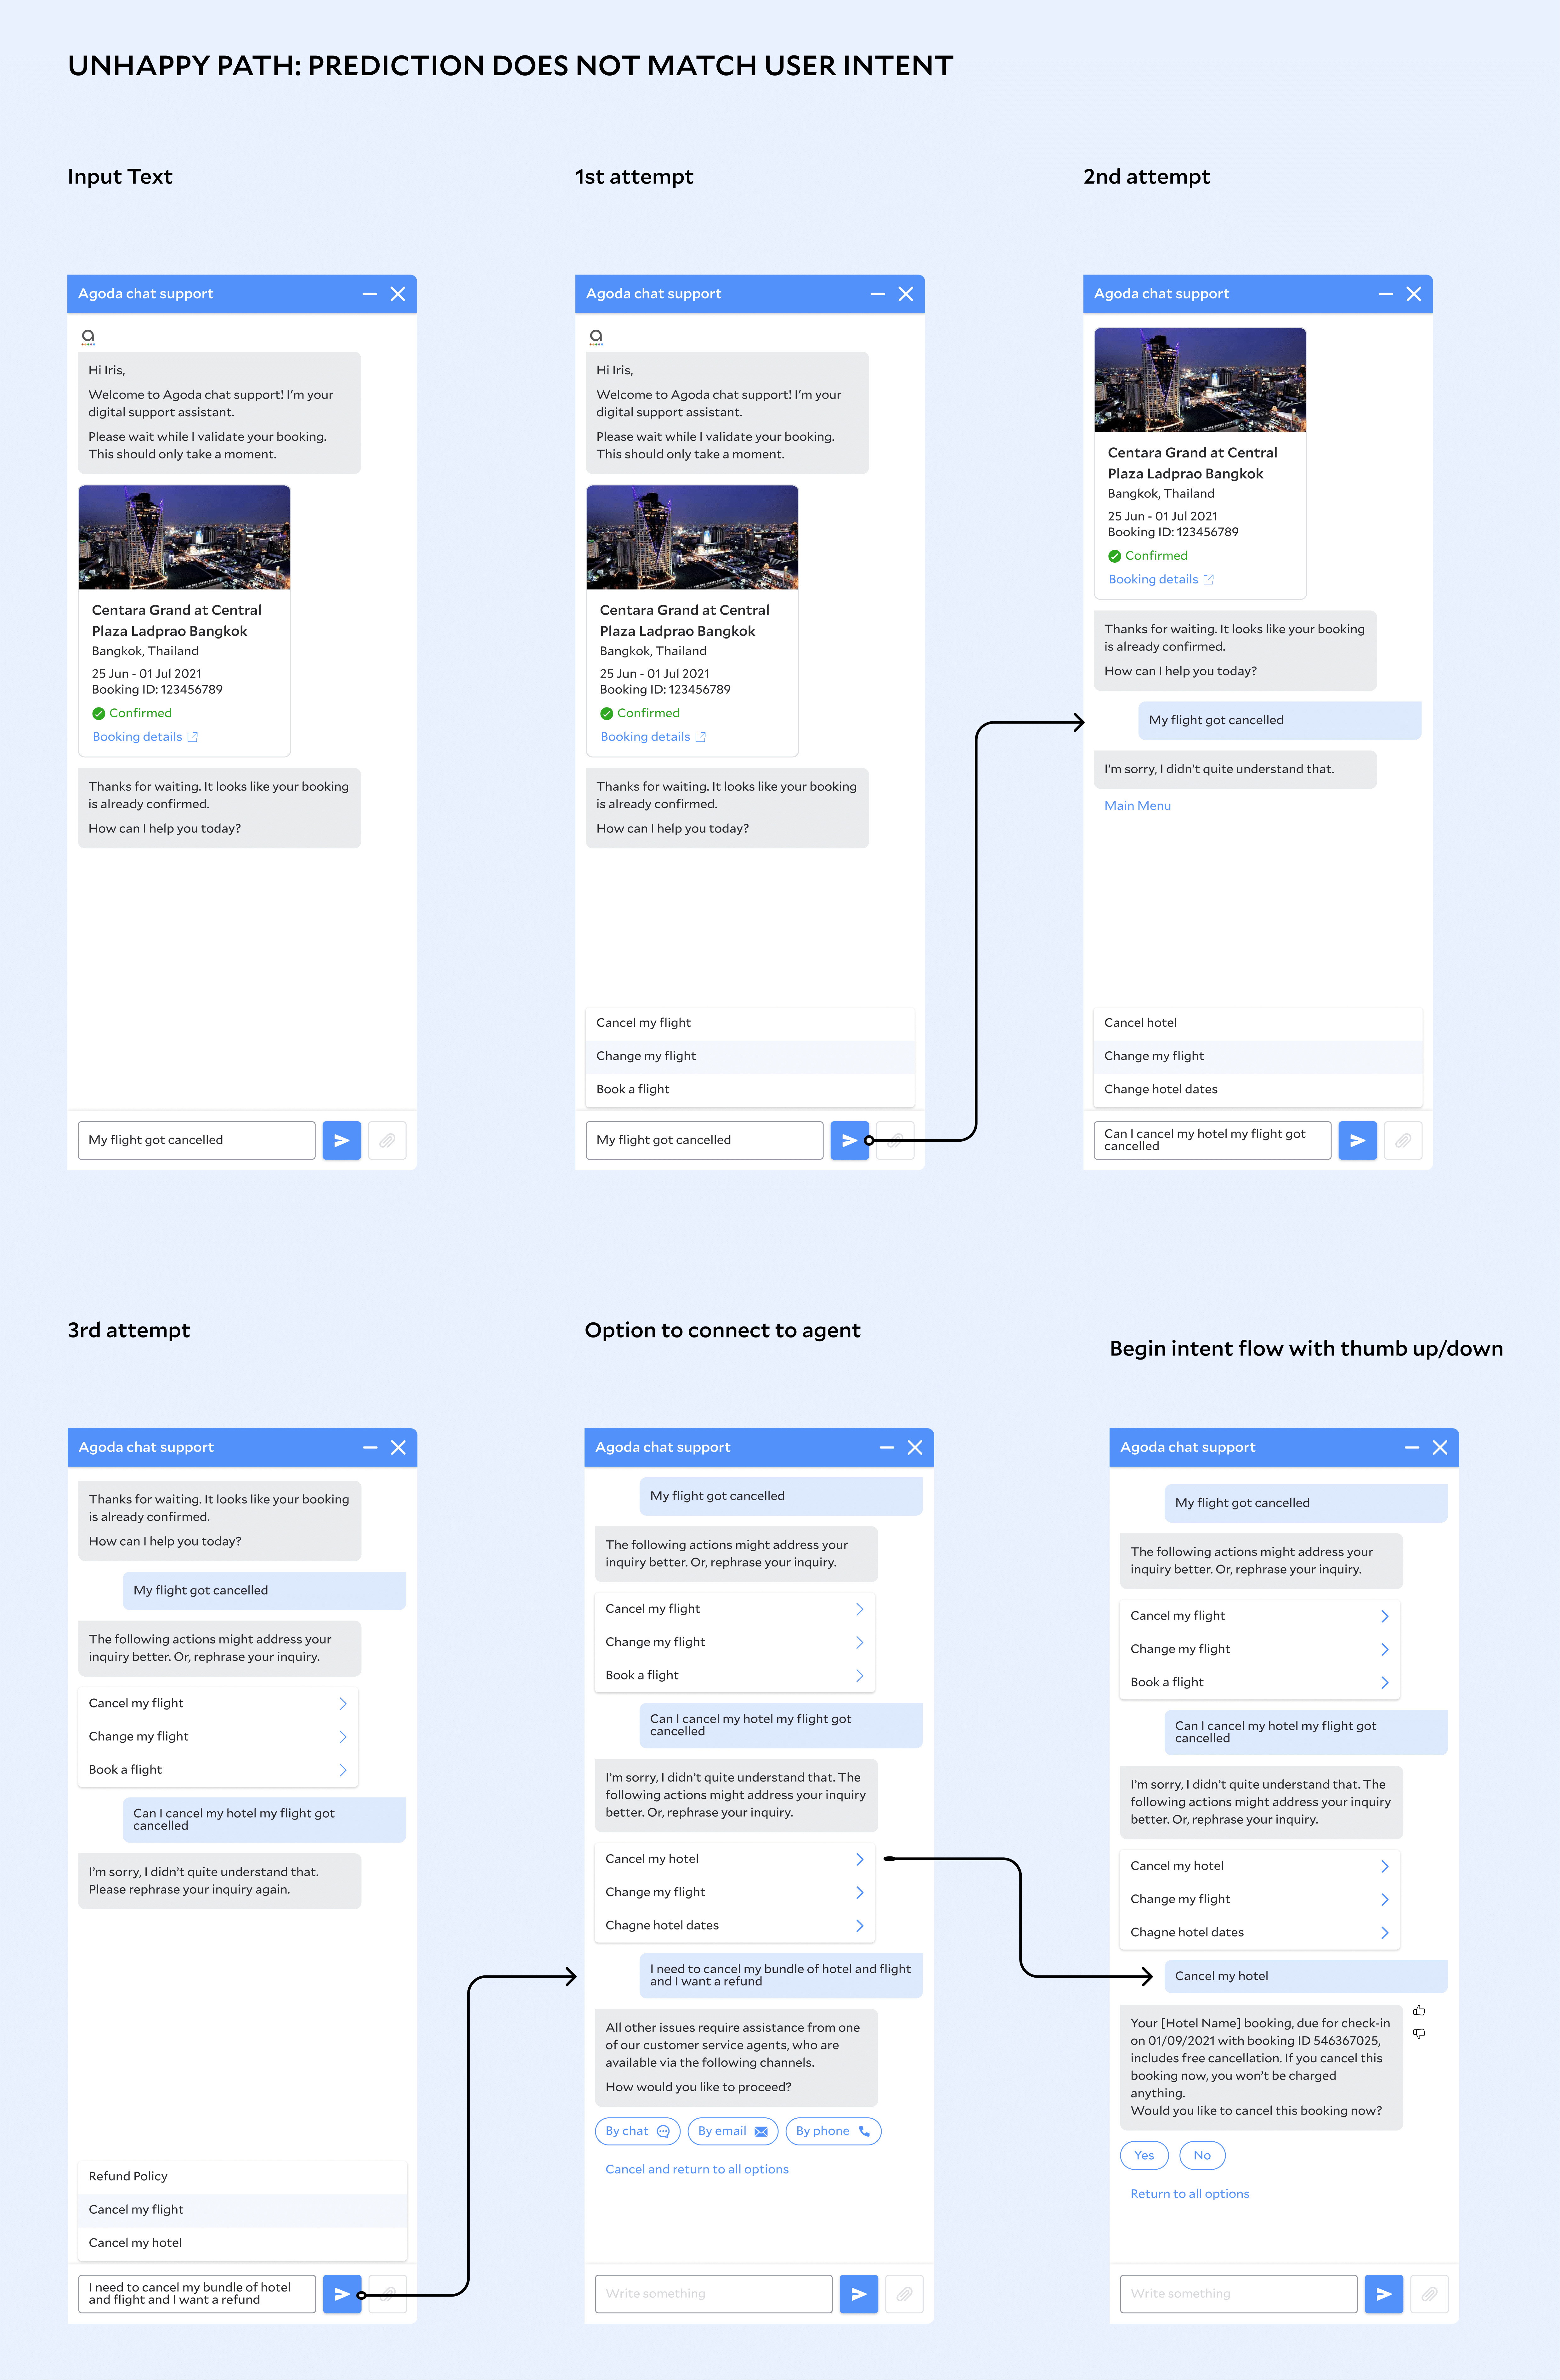
\includegraphics[height=22cm]{jdf-latex/Figures/prototype2.png}
	\caption{User journey to get e-receipt for hotel booking}
	\label{fig:wizard}
\end{figure}
\clearpage

\section{Interface Justification}
From the redesign of the chatbot interface (at the end of this report), we can see that the criticisms from the first section are addressed while preserving the positive elements from the original interface. We have enabled the user to key in free text, and help users to auto-complete sentences if they are not entirely clear about what questions to ask. Also, if the users fail many times by chatbot, the interface will show an option to connect to the real agent.

\subsection{How redesigned interface addresses the requirements from Needfinding}
Through the redesign, the interface now shortens the gulfs of execution and gulfs of evaluation as shown in \textit{\textbf{Table 5}}. The original interface is using the processor view, it assumes 8 pre-defined scenarios for the users (as shown in the \textit{\textbf{Figure 6}}). But the redesigned interface is using the participant view, it considers the user context that will allow users to connect to a real agent if the user query is unique to the context and not able to be addressed by the chatbot itself.

\begin{table}[h] % [h] forces the table to be output where it is defined in the code (it suppresses floating)
	\caption{Gulfs of execution and evaluation}
	\small % Reduce font size
	\centering % Centre the table
	\begin{tabular}{L{0.2\linewidth} C{0.2\linewidth} L{0.2\linewidth} L{0.2\linewidth}}
		\textbf{Name} & \textbf{Stage 1} & \textbf{Stage 2} & \textbf{Stage 3} \\
		\toprule[0.5pt]
		Gulfs of execution & Identify Intentions & Identify Actions & Execute in Interface\\
		\midrule
		Gulfs of evaluation & Interface Output & Interpretation & Evaluation\\
	\end{tabular}
\end{table}

\begin{figure}[hbt!]
	\centering
	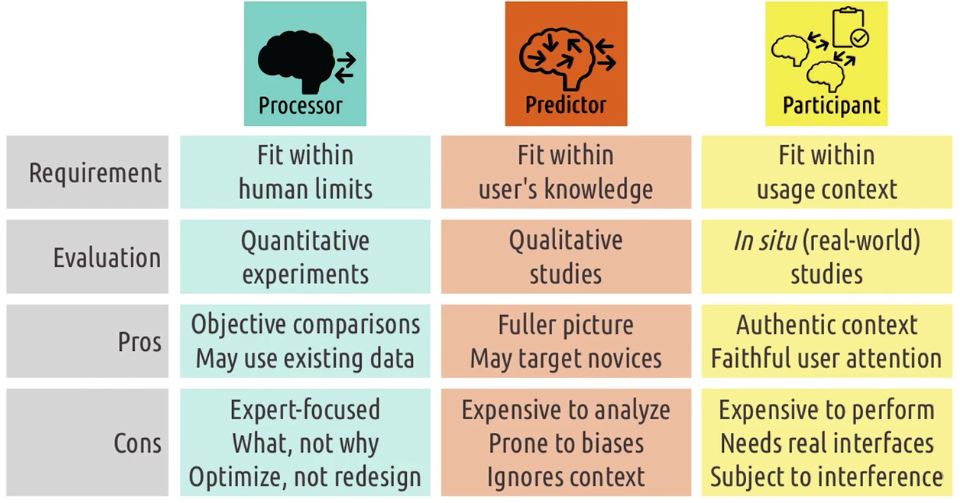
\includegraphics[height=7cm]{jdf-latex/Figures/user_view.png}
	\caption{Processor View, Predictor View, and Participant View}
	\label{fig:wizard}
\end{figure}



\subsection{Summary Table - Issues, Solutions and Design Principles}
\textit{\textbf{Table 6}} summarize all the improvements to address the design principle issues in current interface.
\begin{table}[hbt!]
	\caption{Issues, Solutions in Redesign and Design Principles}
	\small % Reduce font size
	\centering % Centre the table
	\begin{tabular}{L{0.35\linewidth} L{0.15\linewidth} L{0.4\linewidth}}
		\textbf{Original Issues} & \textbf{Design Principles} & \textbf{Redesign Solutions} \\
		\toprule[0.5pt]
		Users are hard to find chatbot interface & Discoverability & We will move the access of chatbot to the home page, users can do one-click access \\
		\midrule
		The normal user input is greyed out and users will be confused by the interface & Affordance & The interface allows free text, users can use the text input box as it is \\
		\midrule
		Users are not able to make mistakes or ask wrong questions & Tolerance & The interface will allow users to ask any questions, and transfer to a real agent if not able to handle the query \\
		\midrule
		Users are not able to ask the real issues they are facing other than the predefined 8 intentions & Flexibility & Free text input is enabled by the interface, users are allowed to ask all kinds of questions \\
		\midrule
		Users will be confusing about what the chatbot interface can do & Consistency & The chatbot interface will have the consistency as other chatbot interfaces to reduce the cognitive effort of users \\
		\midrule
		The interface looks like a chat interface but it only allows follow the pre-defined flow & Mapping & Chatbot interface will be similar to day-to-day chat interfaces like WhatsApp or Telegram, it will bridge the gulfs of execution \\
		\midrule
		The feedback is not helpful if the chatbot does not understand the input query & Feedback & The chatbot will give feedback such as "I don't understand", and transfer to real agent after 2 times failure \\
		\midrule
		Novice users may not need to access chatbot to solve their issues & Expert Blindspot  & A first-timer walk-through will pop up if the user is logging in for the first time. \\
		\midrule
		Users can be frustrated if they are trying to get in touch with real agents & Learned Helplessness & The interface will provide an "exit" option for the user using chatbot and cannot find the answer after many times trying \\
	\end{tabular}
\end{table}
\clearpage

\section{Evaluation Plan}
According to Joyner, \textit{\textbf{Table 7}} are the advantages for different methods: (\cite{joyner2016a})

\begin{table}[hbt!]
	\caption{Advantages for different evaluation methods (\cite{joyner2016a})}
	\small % Reduce font size
	\centering % Centre the table
	\begin{tabular}{L{0.5\linewidth} L{0.1\linewidth} L{0.1\linewidth} L{0.1\linewidth}}
		\textbf{Advantages} & \textbf{Qualitative} & \textbf{Empirical} & \textbf{Predictive}\\
		\toprule[0.5pt]
		Informs ongoing design decisions & Yes & - & Yes \\
		\midrule
		Investigates the participant's thought process & Yes & - & Yes \\
		\midrule
		Draws conclusions from actual participants & Yes & Yes & - \\
		\midrule
		Identifies provable advantages & - & Yes & - \\
		\midrule
		Provides generalizable conclusions & - & Yes & - \\
		\midrule
		Does not require any actual users & - & - & Yes \\
	\end{tabular}
\end{table}

Since the chatbot interface we are studying is an existing interface and we would like to evaluate the performance of the redesigned interface, we will use empirical evaluation to evaluate.

\subsection{Empirical Evaluation}
\textbf{Control Group:} Randomly assigned people, 50\% of the total test population.

\textbf{Experimental Group:} Randomly assigned people, the rest 50\% of the total test population.

\textbf{Null Hypotheses H0:} The redesigned chatbot interface is not significantly better than the original interface.

\textbf{Alternative Hypotheses H1:} The redesigned chatbot interface is significantly better than the original interface.

\textbf{Independent Variables:} The user demographics, the device types, the Geo-locations, dates and all other Agoda app interfaces shall be independent variables that both the control group and experimental group have the same distribution.

\textbf{Dependent Variables:} The only difference between the control group and experimental group is the Chatbot interface of the Agoda app. So the only dependent variable shall be the chatbot interface.

We shall conduct a \textbf{between-subjects} study, daily visitors of the Agoda app are randomly divided into the control group (50\%) and experimental group (50\%) to perform the \textbf{A/B testing}. Since Agoda currently has 75 million active users, a few days of experimentation will give us enough confidence about the outcome. The outcome signal is based on the user interaction by the end of the chatbot flow, whether the user selects "Yes" or "No" to the final question "Is the issue solved?". We will exam the statistical significance (p-value) after the experiment to decide whether to reject the null hypothesis.

\subsection{Planned Statistical Analysis}
We can refer to \textit{\textbf{Table 8}} to select the proper empirical test for the redesigned chatbot interface. Because in this experiment, we have categorical independent variables and binomial dependent variables, we shall use \textbf{Binomial test} to evaluate. If the final result is statistically significant (\textbf{p-value <= 0.05}), we can reject the null hypothesis and conclude that the redesigned chatbot interface is significantly better than the original interface.

\begin{table}[hbt!]
	\caption{Empirical Tests Selection (\cite{joyner2016b})}
	\small % Reduce font size
	\centering % Centre the table
	\begin{tabular}{L{0.2\linewidth} L{0.2\linewidth} L{0.2\linewidth} L{0.2\linewidth}}
		\textbf{IV} & \textbf{DV} & \textbf{Treatments} & \textbf{Recommended}\\
		\toprule[0.5pt]
		Categorical & Nominal & 2 or more & Chi-Squared test \\
		\midrule
		Categorical & Ordinal & 2 & KS test \\
		\midrule
		Categorical & Interval or Ratio & 2 & Student's t-test \\
		\midrule
		Categorical & Ordinal & 3 or more & Chi-Squared test \\
		\midrule
		Categorical & Interval or Ratio & 3 or more & ANOVA \\
		\midrule
		Categorical & Binomial & 1 or 2 & Binomial test \\
		\midrule
		Interval or Ratio & Interval or Ratio & 2 & Linear Regression \\
	\end{tabular}
\end{table}
\clearpage

\section{References}
\printbibliography[heading=none]

\end{document}